\begin{frame}{modifying cache blocks in parallel}
\begin{itemize}
\item cache coherency works on \myemph{cache blocks}
\item but typical memory access --- less than cache block
    \begin{itemize}
    \item e.g. one 4-byte array element in 64-byte cache block
    \end{itemize}
\vspace{.5cm}
\item what if two processors modify different parts same cache block?   
    \begin{itemize}
    \item 4-byte writes to 64-byte cache block
    \end{itemize}
\item cache coherency --- write instructions happen one at a time:
    \begin{itemize}
    \item processor `locks' 64-byte cache block, fetching latest version
    \item processor updates 4 bytes of 64-byte cache block
    \item later, processor might give up cache block
    \end{itemize}
\end{itemize}
\end{frame}

\begin{frame}[fragile,label=paralleModCode]{modifying things in parallel (code)}
\begin{lstlisting}[language=C++,style=smaller]
void *sum_up(void *raw_dest) {
    int *dest = (int *) raw_dest;
    for (int i = 0; i < 64 * 1024 * 1024; ++i) {
        *dest += data[i];
    }
}

__attribute__((aligned(4096))) 
int array[1024];  /* aligned = address is mult. of 4096 */

void sum_twice(int distance) {
    pthread_t threads[2];
    pthread_create(&threads[0], NULL, sum_up, &array[0]);
    pthread_create(&threads[1], NULL, sum_up, &array[distance]);
    pthread_join(threads[0], NULL);
    pthread_join(threads[1], NULL);
}
\end{lstlisting}
\end{frame}

\begin{frame}{performance v. array element gap}
(assuming \texttt{sum\_up} compiled to not omit memory accesses)
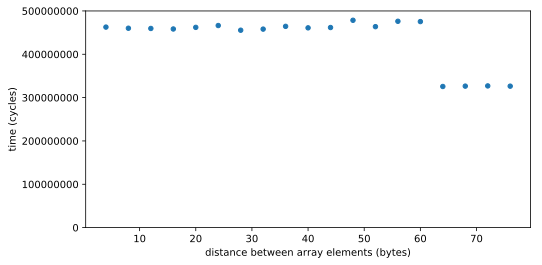
\includegraphics[width=\textwidth]{../sync/sum-up}
\end{frame}

\begin{frame}{false sharing}
\begin{itemize}
\item synchronizing to access two independent things
\vspace{.5cm}
\item two parts of same cache block
\item solution: separate them
\end{itemize}
\end{frame}
